%!TEX root = ../../report.tex
\chapter{Mapping of Static environments}
This chapter investigates improved mapping of static environments with LIDAR sensors by incorporating sensor and localization noise. 
Specifically the following aim is considered:

\begin{enumerate}
    \setcounter{enumi}{0}
    \item Precise mapping of static environments by incorporating sensor and localization noise
\end{enumerate}

Mapping of static environments is an essential part of mobile robotics. It forms the basics for allowing the robot to navigate the environment. 
By integrating measurements with Bayes methods for a short period of time, where the local environment is likely to be static, the effects of sensor and localization errors can be reduced.
Figure \ref{fig:static_map_overview} shows the static mapping module in relation to the rest of the dynamic mapping system.  

\begin{figure}[htbp]
		\centering
		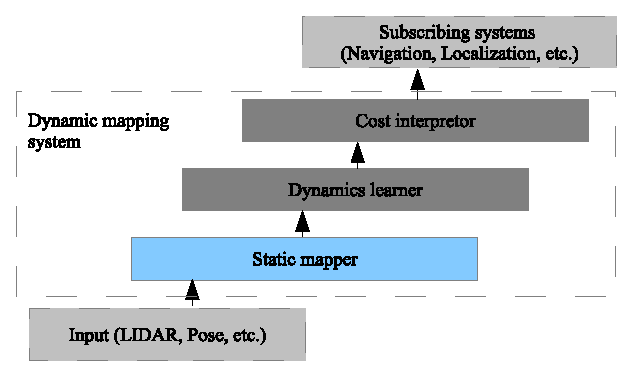
\includegraphics[scale=1]{chapters/static_mapping/figures/static_map_overview.eps}
		\caption{The static mapping in the dynamic mapping system}
		\label{fig:static_map_overview}
\end{figure}


%!TEX root = ../../report.tex
\section{Occupancy grid mapping}

An initial decision in mapping is how to represent the environment. A widely used method is the occupancy grid map, described in \cite{elfesMoravecOccGrid}. It splits the environment into evenly sized cells. Each cell contains an occupancy value describing probability the cell being occupied. 0 for completely free and 1 for completely occupied. An assumption in the occupancy grid map is that each cell is independent which is not strictly true but helps reduce the complexity of the mapping [**REFERENCE INSERT HERE***]. This can be expensive in memory as the entire environment is represented in the grid map. The benefit of the grid map is an ease of maintenance and good metric information \cite{mapbuildingSummary}. 
Another widely used representation is the topological map \cite{topologyOrig}. 
Herein the environment is represented as position or landmark nodes connected by vertices in a graph structure. 
This representation was created for effective navigation in the environment. 
A drawback of the topological map is that it contains less metric information than the occupancy grid mapping \cite{mapbuildingSummary}.

For the static mapping in this project there are other factors influencing the choice of representation. In the ROS system the grid map is already used and therefore the interfacing becomes significantly simpler and thus rendering the proposed mapping more easily integrated in other systems. The availability of metric information and the widespread use and therefore ease of integration makes the occupancy grid a favored choice in this project. 

hen mapping with an occupancy grid each observation is treated as independent and thus adds a contribution to the occupancy of the cell. The most simple mapping in occupancy grid will mark a cell in accordance to its last observation with the full value. If the cell is observed as occupied the cell value is set to 1 and 0 if it is observed free. Using this very simple mapping the last observation is fully in control of the cell value. This makes the method very susceptible to any form of noise. To avoid this, values based on a sensor model are often used to compensates for the noise in the sensor. 

In the occupancy grid a log-odds representation of the probability is used \cite{probRob}. In equation \ref{eq:log-odds} the calculation from probability to log-odds is shown. The value \(p(m_{occ}|z)\) is determined by the sensor model. 

\begin{equation}
\label{eq:log-odds}
l_{occ} =  log(\frac{p(m_{occ}|z)}{1-p(m_{occ}|z)} )
\end{equation}

where \(z\) is the observation and \(m_{occ}\) is the occupied state. 
\\
Using the log-odds representation the occupancy value of a cell is calculated by equation \ref{eq:occGrid_occCalc}. 

\begin{equation}
\label{eq:occGrid_occCalc}
cell_{occ} = \sum_{i} log(\frac{p(m_{occ}|z_i)}{1-p(m_{occ}|z_i)} )
\end{equation}



Why occupancy grid ? (interface, recognised, used through put the community - considerations on other representation)
Mapping by inserting obstacle and free when observed.
Independence - cells, measurements
Log odds
Real world test -> Results in bad maps.
Propagation of noise to avoid over confidence while still converging to the right solution. (Types of noise)


%!TEX root = ../../report.tex
\section{Laser range sensor}

Basics of sensor
Forward Sensor Model
What noise does the sensor introduce. (see prob robotics)
Ideal Inverse Sensor Model

Elfes Sensor Model
Reference to Elfes
Calculated through kernel density estimation. 
Considerations on the std deviation

%!TEX root = ../../report.tex
\section{Mapping with Location noise}

\subsection{Monte Carlo localization}

AMCL

Scan map with location noise and AMCL
Considerations on noise. What types of noise are present. Estimation of the noise. Comparison between estimation and actual error (of bags) 
Non-ideal Inverse Sensor Model
From hector

\subsection{Monte Carlo Integration Inverse Sensor Model}

\cite{monteCarloIntegration}

Cone Sensor Model
Based on sonar model. Used to incorporate pose noise. 
Simulation of Mapping with Location Noise
Comparison
Efficiency - Computational price
Map Score (obstacle centered and whole map, adjusted for number of cells)
\begin{figure}
	\centering
	\includegraphics[width=0.7\linewidth]{figures/static_mapping/particle_sensor}
	\caption{Example map with few scans from the five highest weighted particles.}
	\label{fig:particle_sensor}
\end{figure}

\begin{figure}
	\centering
	\begin{subfigure}[b]{0.45\textwidth}
		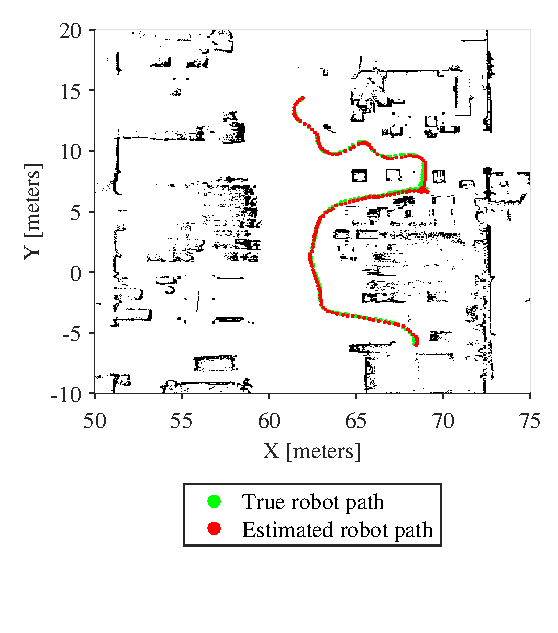
\includegraphics[width=\textwidth]{figures/static_mapping/map_with_poses}
		\caption{World represenation}
		\label{fig:simulated_robot_estimate_total}
	\end{subfigure}
	~ %add desired spacing between images, e. g. ~, \quad, \qquad, \hfill etc. 
	%(or a blank line to force the subfigure onto a new line)
	\begin{subfigure}[b]{0.45\textwidth}
		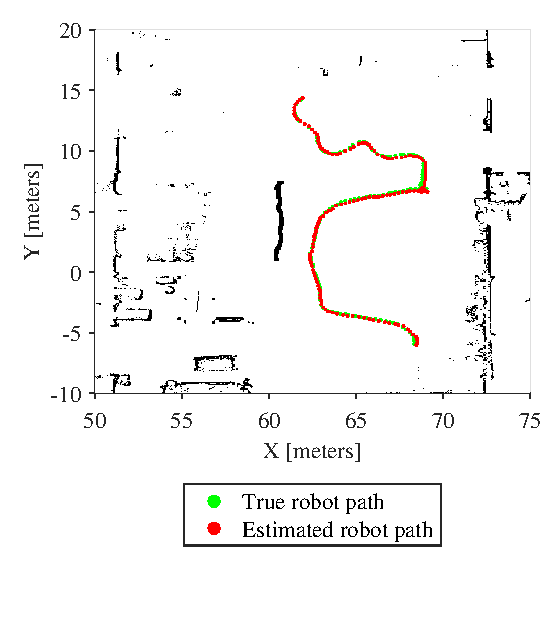
\includegraphics[width=\textwidth]{figures/static_mapping/amcl_map_with_poses}
		\caption{Map used by AMCL}
		\label{fig:simulated_robot_estimate_total_edited}
	\end{subfigure}
	\caption{Simulation of a MIR robot moving with imprecise location.}
	\label{fig:animals}
\end{figure}


%!TEX root = ../../report.tex
\section{Mapping an Industrial Environment}

Test setup 
Something about the scan environment
Mapping of the scan environment

Results

Conclusion

Observation: Jumps in localisation - must be considered and possibly suppressed

%!TEX root = ../../report.tex
\section{Summary}
In this chapter various different methods of including pose estimation noise into the mapping has been evaluated. The method that was ultimately chosen was in ideal sensor model but with reduced certainty for each observation. The occupancy values chosen for free is \(0.4\) and \(0.6\) for occupied. The pose estimation noise in incorporated as a weight that reduces the certainty as the estimation variance increases. The weight calculation can be seen in equation \ref{eq:pose-weight}. 
These elements has been inserted in the static mapper block, as seen in figure \ref{fig:static_map_detail}. 
The sensor input and pose estimation is combined and inserted in the static map as determined by the sensor model and noise weight. At fixed intervals the static map is then provided as a snapshot as output and cleared. 

\begin{figure}[htbp]
	\centering
	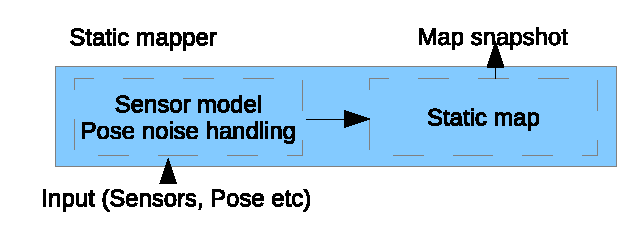
\includegraphics[scale=1]{chapters/static_mapping/figures/static_map_detail.eps}
	\caption{Static mapping module concept}
	\label{fig:static_map_detail}
\end{figure}

